\documentclass[12pt]{article}

\usepackage{fullpage}
\usepackage{graphicx, rotating, booktabs} 
\usepackage{times} 
\usepackage{natbib} 
\usepackage{indentfirst} 
\usepackage{setspace}
\usepackage{grffile} 
\usepackage{hyperref}
\usepackage{adjustbox}
\usepackage{amsmath}
\usepackage{siunitx}
\usepackage{multirow}
\setcitestyle{aysep{}}


\singlespace
\title{\textbf{Democracy, Elections, and Alliance Treaty Depth}}
\author{Joshua Alley\footnote{Postdoctoral Research Associate,
University of Virginia.}}
\date{\today}

\bibliographystyle{apsr}

\begin{document}

\maketitle 

\doublespace 

\begin{abstract}
Why do states form deep alliance treaties, which reinforce military support promises with commitments of defense coordination and cooperation? 
I argue that democratic alliance leaders use treaty depth to make more credible alliance commitments in the face of leadership turnover. 
Electoral democracy can empower leaders with less commitment to an alliance. 
Such leadership turnover threatens credible commitment by democracies. 
Therefore, incumbent leaders use treaty depth to make reduced alliance commitment more costly. 
Thus, electoral democracy in the most capable alliance member leads to greater treaty depth.
I test this claim on offensive and defensive alliances from 1816 to 2007 and illustrate the theoretical mechanisms by examining NATO.
I find that greater electoral democracy in the most capable alliance member increases treaty depth. 
The argument and findings provide insight into the connection between domestic politics and the design of international institutions. 
\end{abstract}


\newpage 


\section{Introduction}


% Start with question and motive 
Why do states make deep alliance treaties? 
Deep alliances formalize extensive defense cooperation by using additional military policy coordination and cooperation in to supplement promises of military intervention. 
While shallow alliances offer arms-length military support, deep treaties lead to closer ties between alliance members. 
Key sources of depth include an integrated military command, military aid, a common defense policy, basing rights, international organizations, and companion military agreements, and half of all offensive and defensive alliances\footnote{Treaties that promise active military support.} include at least one source of depth \citep{Leedsetal2002}. 
Despite the prevalence of alliance treaty depth, we have little idea when states add depth to their alliances. 


% Generalize: IO design is not just primary commitments, but how states support/implement their promises
Understanding the sources of deep alliances is worthwhile for two reasons.
First, depth shapes alliance credibility and the distribution of military spending among alliance members. 
Costly commitments in deep alliances increase the credibility of military support promises \citep{Morrow1994}, which then encourages non-major power members of deep alliances to reduce military spending \citep{Alley2020}.  
Second, the process behind alliance treaty depth may provide more general insights into international institution design. 
Members of international organizations often use costly commitments to support cooperation. 
For example, some trade agreements use third-party dispute settlement mechanisms to enforce agreements \citep{Smith2000}, or institutionalize formal monitoring arrangements \citep{Duretal2013}.  
Understanding when and why states employ close or arms-length cooperative commitments is therefore worthwhile. 


% Describe question and contribution of the paper
In this paper, I argue that democratic alliance leaders use treaty depth to increase the durability of their alliance commitments in the face of leadership turnover. 
Although the leader negotiating an alliance has high alliance commitment, elections could empower less committed leaders and threaten credible commitments \citep{GartzkeGleditsch2004, LeedsSavun2007}.
In anticipation of this turnover threat, incumbent leaders can use treaty depth to ensure help their successors signal alliance reliability and make reducing an alliance commitment more difficult and costly. 
Therefore, I expect that electoral democracy in the most capable alliance member leads to deep alliance treaties. 


So long as voters support alliance formation, opposition leaders will have limited capacity to veto treaty depth. 
Executive constraints, another salient component of democratic institutions, do give opposition elites some influence to limit treaty depth at the margins, however.
Thus, the net effect of competitive elections and executive constraints in democracies is increased treaty depth in alliances with a democratic leader.  


% describe the test
I test the argument with a statistical analysis of offensive and defensive alliances from 1816 to 2007 and then examine the theoretical mechanisms in the context of NATO treaty design.
I find consistent evidence that greater electoral democracy in the alliance leader increases treaty depth. 
The results are robust to different model specifications and samples, as well as several multiple equation estimation techniques. 


% Two Paras on the gap I fill 
This paper contributes to knowledge of alliance treaty design and how domestic politics affects alliance choices.
Democracy affects alliance politics in many ways \citep{LaiReiter2000, GiblerWolford2006, Mattes2012a, Warren2016, McManusYarhi-Milo2017}. 
Connecting domestic electoral institutions and treaty depth adds to this scholarship and addresses an important gap.
The process of alliance treaty negotiation and design is understudied \citep{Poast2019a}, and there is little research on treaty depth because the nascent alliance treaty design literature emphasizes conditions on military support.
Existing research identifies entrapment concerns \citep{Kim2011, Benson2012} and democratic alliance membership \citep{Mattes2012, Chibaetal2015} as two sources of conditional obligations.\footnote{\citet{FjelstulReiter2019} supplement research on support conditions by arguing that democracies use incomplete alliance contracts to limit audience costs.} 


Two studies of alliance treaty design examine similar concepts to treaty depth, but both have important limitations.   
First, \citet{Mattes2012} finds that members of symmetric bilateral alliances where one partner has history of violation are more likely to use military institutionalization to increase treaty reliability. 
This paper makes an important contribution, but it only analyzes bilateral alliances and uses an ordinal military institutionalization measure by \citet{LeedsAnac2005} that understates variation in treaty depth.  
Second, while checking the validity of a latent measure of costly alliance obligations, \citet{BensonClinton2016} find that foreign policy agreement, major power involvement and treaty scope increase depth. 
Benson and Clinton define depth as how costly alliance obligations are in general, however, so their latent measure of depth includes secrecy and issue linkages and captures a broader concept than defense cooperation. 


Therefore, we still do not understand why alliance members employ treaty depth.
To address this lacuna, I consider how domestic political institutions and potential leadership turnover shape institutional design.
Democratic leaders add depth to alliances to maintain credible commitment by future leaders with different constituencies.  
Thus, leaders strategically employ different foreign policy tools within their institutional context \citep{HydeSaunders2020}. 


% implications: 
There are two primary implications of my argument and findings. 
First, they add important nuance to existing claims that democracies prefer limited alliance commitments \citep{Mattes2012, Chibaetal2015, FjelstulReiter2019}. 
Even as democracies screen the breadth of conditions on military support, they form deeper alliances in other ways.
Furthermore, the findings add to the rich literature on domestic politics and international cooperation e.g. \citep{DownesRocke1995, Fearon1998, Leeds1999, MattesRodriguez2014}. 
Just as democracies reassure partners with deep alliance commitments, electoral politics may push democracies to undertake strong international commitments with conditional primary obligations.\footnote{For example, in environmental agreements, democracies may prefer soft law commitments \citep{BoehmeltButkute2018}, but other aspects of these agreements may be deep and less salient.} 


% roadmap for the paper 
The paper proceeds as follows. 
In the next section, I lay out the argument and hypotheses. 
Then I summarize the data and research design. 
After this, I describe the results and detail U.S. alliance treaty design considerations in NATO negotiations.
In the final section I summarize the results and offer some concluding thoughts. 


\section{Argument}


In this argument, I first consider role of domestic politics in alliance negotiations. 
I then explain how leadership turnover in alliances threatens treaty credibility. 
Last, I consider how depth addresses credibility concerns from regular leadership turnover. 


% explain allliances
Alliances are self-enforcing contracts or institutions where states promise military intervention \citep{Leedsetal2002, Morrow2000}. 
When faced with external threats in an anarchic international system, states form alliances to aggregate military capability and secure their foreign policy interests \citep{Altfield1984, Smith1995, Snyder1997, FordhamPoast2014}.
Alliance participation has several costs and benefits.
Beyond the benefit of possible military support, alliances also clarify international alignments \citep{Snyder1990} and support economic ties \citep{Gowa1995, Li2003, Long2003, Fordham2010, WolfordKim2017}.  
The costs of alliance participation include opportunism and lost foreign policy autonomy \citep{Altfield1984, Morrow2000, Johnson2015}. 
Opportunism in alliances has three forms; abandonment of military intervention promises \citep{Leeds2003a, BerkemeierFuhrmann2018}, entrapment in unwanted conflicts \citep{Snyder1984}, and free-riding \citep{Morrow2000}.


% process of alliance negotiations: establishing a credible commitment. 
To form an alliance, states must have similar foreign policy interests \citep{Morrow1991, Smith1995, FordhamPoast2014}. 
\citep{Poast2019a} notes that agreement over a treaty in alliance negotiations depends on outside options and compatible war plans. 
Alliance treaties formalizing promises of military support take many forms \citep{Leedsetal2002, BensonClinton2016}. 
Treaty design shapes the costs and benefits of treaty participation and addresses potential opportunism.  
In the face of abandonment concerns, alliance members use formal commitments to increase the credibility of military intervention promises, as the costs of the alliance commitment provide indications of reliability \citep{Morrow2000}.


% Product of negotiations and domestic constraints
Most studies of alliance treaty design focus on negotiations between states, but as in other foreign policy domains, leaders in alliance negotiations are playing a two-level game \citep{Putnam1988}. 
Alliance agreements reflect both international and domestic political constraints on leaders. 
To give two examples, audience costs concerns shape conditions on military support in alliances between democracies \citep{Chibaetal2015, FjelstulReiter2019}, and whether democratic dyads form consultation or defense pacts depends on the risk of the current leader losing office \citep{Mattes2012a}. 


% Actors in the argument 
Given the importance of domestic politics, there are four key actors in this explanation of the sources of alliance treaty depth. 
First, incumbent leaders seek to form an alliance that offers a credible and durable promise of military support. 
Potential allies consider the credibility of the alliance--- whether it will increase their security. 
In domestic politics, opposition elites and voters could check the foreign policy goals of the incumbent. 
I assume that opposition elites are more likely to oppose alliance formation, but vary in the strength of their objection to an alliance. 
I also assume that voters focus on whether to extend an alliance or not, and pay less attention to treaty design.


% Perspective of the alliance leader 
This argument focuses on domestic politics in the most capable alliance member. 
Highly capable states use alliances to increase their influence abroad, often by protecting smaller states \citep{Morrow1994}. 
As they do so, they must design credible alliance treaties that are viable in domestic politics. 


% Sources of democratic influence in alliance negotiations. 
Furthermore, more capable states have greater influence on alliance negotiations \citep{Mattes2012}, because their partners lose out on foreign policy benefits without their participation.
The most capable state is often the alliance ``leader,'' and their preferences carry more weight. 
Therefore, the domestic institutions of the most capable alliance member are a crucial determinant of alliance treaty design.\footnote{Emphasizing the influence of the largest state is further supported by evidence that the preferences of powerful capital-exporting states drive the design of bilateral investment treaties \citep{AlleePeinhardt2014}.} 


\subsection{Leadership Turnover and Alliance Credibility}


% credibility depends not just on the alliance, but domestic politics
Leaders must account for domestic politics in their efforts to establish credible treaty commitments.
When an alliance is invoked, leaders decide whether to honor or violate the treaty obligations. 
That decision depends in part on domestic concerns, as leaders consider and respond to the views of the coalition that put them in office. 


% leadership turnover- threat to reliability
Leadership turnover can therefore threaten alliance reliability.
New ruling coalitions often implement a different foreign policy \citep{Lobell2004, Narizny2007}.  
Changes in political regimes \citep{LeedsSavun2007}, or the coalitions backing a leader \citep{Leedsetal2009} both increase the risk of alliance treaty abrogation. 
Even as the incumbent negotiating an alliance supports treaty participation, if leadership change empowers an alliance skeptic, the state will be more likely to leave or violate an alliance.  


% institutions shape leadership turnover frequency and regularity
Domestic political institutions shape the frequency and regularity of leadership turnover by structuring how leaders are selected and replaced. 
Some institutions formalize frequent leadership changes, by regularly providing opportunities to select new leaders. 
Others institutions give make leadership without undoing the regime itself difficult at best. 


% democracies have higher risk of leadership change
Democracies have regular leadership turnover. 
Competitive elections for leadership are perhaps the defining feature of democracies, and elections often create different ruling coalitions. 
At a minimum, competitive elections with a viable opposition, multiple candidates and more than one legal party have potential for leadership change \citep{HydeMarinov2012}. 
As the franchise expands, opposition leaders have more potential coalitions they can use to unseat the incumbent.  
Thus, electoral democracy raises the prospect of cycling between different coalitions, which could have different material and ideological foreign policy interests. 
Such cycling may reduce the reliability of democratic alliance commitments through leadership turnover \citep{GartzkeGleditsch2004}.\footnote{See \citet{Gaubatz1996} for a skeptical take on the problem of cycling for democratic reliability.}


% democratic allies can understand this risk 
Democratic allies understand the risk of leadership turnover for treaty reliability. 
Although the leader they are negotiating with supports an alliance, future leaders may not. 
For states seeking a durable alliance commitment, new leaders in a democracy are a potential problem. 
If the alliance is to provide support over the long run, leadership turnover threatens alliance credibility.


% challenge for leaders
Thus, when democratic leaders negotiate an alliance treaty, they must consider what will happen when they leave office.
Establishing credible alliance commitments for democracies requires attention to leadership turnover. 
Given the stakes of an alliance, verbal assurances that future leaders will honor the treaty are likely inadequate.
Allies will require greater reassurance that leadership changes will not undo the alliance. 



\subsection{Credible Commitment through Deep Alliances}

% democracies can address 
Treaty depth is one way for democracies to address the threat of leadership turnover to treaty reliability. 
Depth generates credible commitments through sunk costs.
Regular sunk costs in deep alliances also address the time-inconsistency concerns at the heart of potential leadership changes.


% depth 
Sunk costs in treaty depth help alliance members establish credible commitments.
In a deep alliance, states supplement military support promises with commitments of peacetime cooperation like bases, military aid, policy coordination and formal institutions. 
For example, Treaty of Lisbon between European Union members reinforces defensive support promises with commitments to a common defense policy and funding a European Defense Agency. 
Depth adds to the perceived reliability of an alliance by providing opportunities for states to fulfill peacetime treaty obligations \citep{Morrow1994}. 
Implementing deep treaty obligations is a sunk cost signal of commitment.
Observing that alliance members adhere to peacetime promises suggests that they will also honor promises of military support.\footnote{\citet{LeedsAnac2005} find that alliances with high military institutionalization are less likely to be honored in war, which contradicts this claim that depth increases credibility. 
This finding has two limitations, however. 
First, observed challenges to an alliance may indicate lower credibility \citep{Smith1995}, so there is a selection problem with these estimates, which Leeds and Anac acknowledge. 
Second, their inferences depend on an ordinal measure of alliance treaty depth that limits variation in depth. 
When I employ a continuous latent depth measure in Leeds and Anac's model of alliance fulfillment in offense and defensive alliances, the depth coefficient is positive. 
I find similar results with another model of alliance fulfillment in war using data from \citet{BerkemeierFuhrmann2018}.
See the appendix for details.} 


% depth and turnover: 
Depth also addresses leadership turnover concerns in two ways. 
First, maintaining depth requires continued sunk costs.
Upholding aid, defense cooperation, and basing rights means allies must continue to invest in defense cooperation throughout the life of an alliance. 
When new leaders uphold deep alliance provisions, they send the same signals of reliability as their predecessors. 


% makes adjusting/reducing commitment more costly
Second, depth makes adjusting or reducing an alliance commitment more costly for new leaders. 
Formalizing defense cooperation means that leaders break treaty obligations if they reduce defense cooperation. 
This is in turn exposes new leaders to public and elite disapproval for violating international obligations, so long as the public is paying attention \citep{Slantchev2006, PotterBaum2014} and prefers compliance \citep{Chaudoin2014, KertzerBrutger2016}.


% legalization here


% address issue of rhetoric
These mechanisms help establish credibility even if a leader expresses rhetorical skepticism about an alliance. 
Relative to continuing costly cooperation in an alliance, talk is cheap. 
So long as a leader honors deep alliance obligations, their rhetoric will have a more limited impact on alliance credibility. 




\subsection{Domestic Constraints on Depth} 

% depth is part of domestic pol process 
Like all other alliance components, depth is subject to domestic political constraints. 
The ability of a leader to form a deep alliance depends on opposition and voter preferences.
Elites and voters vary in how detailed their alliance policy preferences are. 
When voters support alliance formation, they are unlikely to check treaty depth.\footnote{This implies that a selection process is present, which I account for in one statistical model in the empirical section.} 
Opposition elites may agree with the incumbent, disagree about treaty design, or oppose alliance formation altogether. 


% domestic opponents may agree
A shared perceived threat, foreign policy consensus, or other factors may lead opposition elites to agree with incumbents on alliance treaty design. 
Thus, opposition elites will have few concerns with treaty depth, and may even welcome depth as a check on future coalitions that empower alliance opponents. 
In these cases, leaders face few domestic constraints on treaty depth. 


% alliance oppponents/out of power folks understand this
Alliance opponents have incentives to check treaty depth, however.
They can anticipate the consequences of treaty depth for their foreign policy flexibility should they win office.
When elites oppose an alliance, they will not support a deep alliance treaty.  
Executive constraints, which are a key factor in democratic foreign policy, increase the potential influence of alliance opponents over treaty design.   
In addition to competitive elections, many democracies check the power of the executive with coequal branches of government, especially courts or legislatures.
For example, legislative ratification of alliance treaties gives other branches of government treaty design input. 


% but usually inadequate
Although executive constraints increase the potential influence of alliance skeptics, they are unlikely to lead to shallow alliance treaties. 
So long as the incumbent has enough support for alliance formation from voters, alliance opponents will have limited influence over treaty depth. 
When the incumbent has popular support, opponents have limited power to use the threat of electoral punishment as a check on treaty depth. 


% explain further- how
%Incumbent leaders may be able to win the support of some alliance opponents by making more limited alliance commitments.
%This assumes that alliance skeptics vary in the intensity of their opposition.  
%While some alliance skeptics will oppose any treaty, others may support an alliance, so long as it has limited obligations that retain future flexibility. 
%While building support for an alliance, a constrained executive may drop some treaty depth in exchange for support from marginal alliance skeptics. 


% voters are unlikely to punish depth, conditional on supporting the alliance. 
Moreover, when voters support alliance formation, they are unlikely to disapprove of treaty depth.
In fact, voters may see close cooperation with allies as appropriate. 
Therefore, voters are unlikely to restrain treaty depth, conditional on approval of the alliance itself. 
If a leader has enough support to negotiate and form an alliance, public opinion is unlikely to check treaty depth. 


% this implies selection
Domestic constraints clearly show a non-random selection process for observed alliances. 
When an incumbent has domestic support for alliance formation, they can also offer a deep alliance treaty. 
A domestic coalition behind an alliance could reflect agreement between the opposition and leading elites, or limited opposition power to offset voter support. 
Limited voter concerns over the specifics of alliance treaty design attenuates the ability of opposition elites to restrict depth and alliance commitments.
Opposition elites may be able to mobilize coalitions to block alliance formation, but if that fails, they will lack influence to do more than limit depth at the margins. 



\subsection{Predictions}

% What is it exactly about democracies?
Democratic institutions lead to deeper alliances as leaders seek to manage the problem of cycling. 
Elections encourage incumbent leaders in democracies to form deep alliances.
Selecting leaders through elections raises the prospect of leadership turnover and cycling that limits the ability of a democracy to sustain credible commitments. 
Elections are therefore the key characteristic of democracy for understanding treaty depth. 
As noted earlier in the argument, I conceptualize democratic influence in terms of the political institutions of the most capable alliance member.


% the extent of electoral democracy- elections, competition, franchise
The extent of electoral democracy in an alliance leader depends on the presence of elections, meaningful electoral competition, and enfranchisement. 
Elections and competition raise the potential of regular leadership turnover. 
Full enfranchisement creates the possibility of greater cycling, as elections are more likely to empower different coalitions under a broad franchise. 


% express the depth and elections hypothesis
Because depth helps address cycling concerns from leadership changes, democracies will often design deep alliance treaties. 
Therefore, greater electoral democracy in the most capable alliance member at the time of treaty formation will increase treaty depth. 


\begin{quote}
\textsc{Electoral Democracy Hypothesis: Greater electoral democracy in the most capable alliance member at the time of formation will increase alliance treaty depth.}
\end{quote}   


% deal with audience costs argument- quick compare/contrast 
This argument is slightly different from existing arguments linking democracy and alliance treaty design, which rely on the audience costs of future treaty violations. 
\citet{Mattes2012} and \citet{Chibaetal2015} attribute democratic states' preference for conditional military support to careful audience costs management. 
In this argument, democratic leaders make limited commitments that are easier to fulfill in anticipation of removal from office from violating international commitments.\footnote{See \citet{HydeSaunders2020} for a more general framework of domestic constraints on foreign policy.} 
Limiting alliance commitments through conditional military support reduces audience costs because it is easier for democratic leaders to claim that the conditions for intervention were not met \citep{FjelstulReiter2019}, or that new information eliminates intervention obligations \citep{LevenduskyHorowitz2012}. 


% discuss these two arguments
The electoral democracy and audience costs arguments have some similarities and important differences. 
One reason treaty depth limits cycling in alliance commitments is that leaders may pay audience costs for violating deep alliance provisions. 
Rather than restrict audience costs to specific conditions, depth raises potential audience costs for future leaders with different interests. 
Depth allows leaders to make costly alliance commitments that precommit their successors to the alliance \citep{Mattes2012a}. 
In an audience costs argument, leaders fear that future treaty violations will weaken their electoral support, and reason backwards from this to alliance treaty design. 
Electoral politics relies on incumbents anticipating a change in the ruling coalition, and seeking to maintain credible alliance commitments.\footnote{Leadership turnover might factor into democracies' tendency to offer conditional support. Leaders may use conditional support to ensure that their successors will fulfill alliance obligations.} 


% What about different types of autocracies?: can omit. 
My argument uses electoral competition to explain why democracies often form deep alliances. 
What about autocracies? 
There is substantial variation in how autocracies select leaders. 
For example, in single-party states, leaders rely on support from domestic elites, which affects their foreign policy decisions \citep{Weeks2014}.
Elite turnover in single party states usually keeps the same coalition in power, however.  
Leadership change in personalist regimes is more likely to be irregular and include regime change.
Treaty depth is unlikely to maintain an alliance after regime change.  
In general, no autocracy has the same concern of regular cycling between different coalitions as democracies.
Therefore, assuming that all autocracies are equivalent, relative to democracies is sufficient for testing the electoral politics argument.\footnote{Examining heterogeneity among autocracies in alliance treaty design is an interesting subject for future research, however.} 


% because depth and uncond milsup are related, correlated choices
I expect that democratic alliance leadership will increase treaty depth through competitive elections. 
In the next section, I describe my test of the association between democratic alliance leadership and alliance treaty design. 
I first describe the key variables in the analysis, then provide more detail on the estimation strategy.



\section{Research Design}



% start with data
To examine whether democracies are more likely to form alliances, I employ data from the Alliance Treaty Obligations and Provisions (ATOP) project \citep{Leedsetal2002}. 
The analysis focuses on the design of 289 alliances with either offensive or defensive obligations.\footnote{Results are robust to adjusting for non-random selection into alliances. See the appendix for details.}
First, I measure treaty depth in these alliances with active military support. 


I measure treaty depth with a semiparametric mixed factor analysis of eight ATOP variables \citep{Murrayetal2013}.
This measurement strategy has two advantages. 
First, unlike other measures, this approach captures the full spectrum of variation in defense cooperation across alliances.
This latent variable approach is more flexible than an ordinal measure \citep{LeedsAnac2005} and more focused on defense cooperation than another latent measure \citep{BensonClinton2016}.\footnote{See the appendix for results with measures by \citet{LeedsAnac2005} and \citet{BensonClinton2016}, which lead to similar inferences. I also discuss the relative advantages of my measure in more detail.}
Besides matching my conceptualization of treaty depth, the estimator relaxes distributional assumptions about the correlation between the factors and latent variable, making it more flexible and robust than other factor analytic models. 
Added flexibility from the semiparametric component aside, this model is a standard mixed Bayesian factor analysis. 
Based on the argument, I fit the model with a single latent factor, and the results corroborate this expectation.\footnote{This is a confirmatory factor analysis, not an exploratory analysis.}
An eigenvalue decomposition of the posterior mean correlations between the observed variables suggests that one latent factor explains most of the observed variation in the different sources of treaty depth.\footnote{Also, a model with one latent factor converges, while a model with two factors does not converge. Such model-fitting difficulties can indicate misspecification.} 


My depth measure is essentially a weighted combination of ATOP's defense policy coordination, military aid, peacetime integrated military command, formal organization, companion military agreement, specific contribution, wartime subordination and basing rights variables.
The weight of each variable is estimated by the measurement model, so it is driven by the data.  
All eight variables increase alliance treaty depth, but defense policy coordination and an integrated command add the most to depth, as shown in the top panel of \autoref{fig:loadings-measure}. 
Thus, policy coordination and formal organizational ties are the primary sources of treaty depth. 


\begin{figure}[hbtp]
\centering
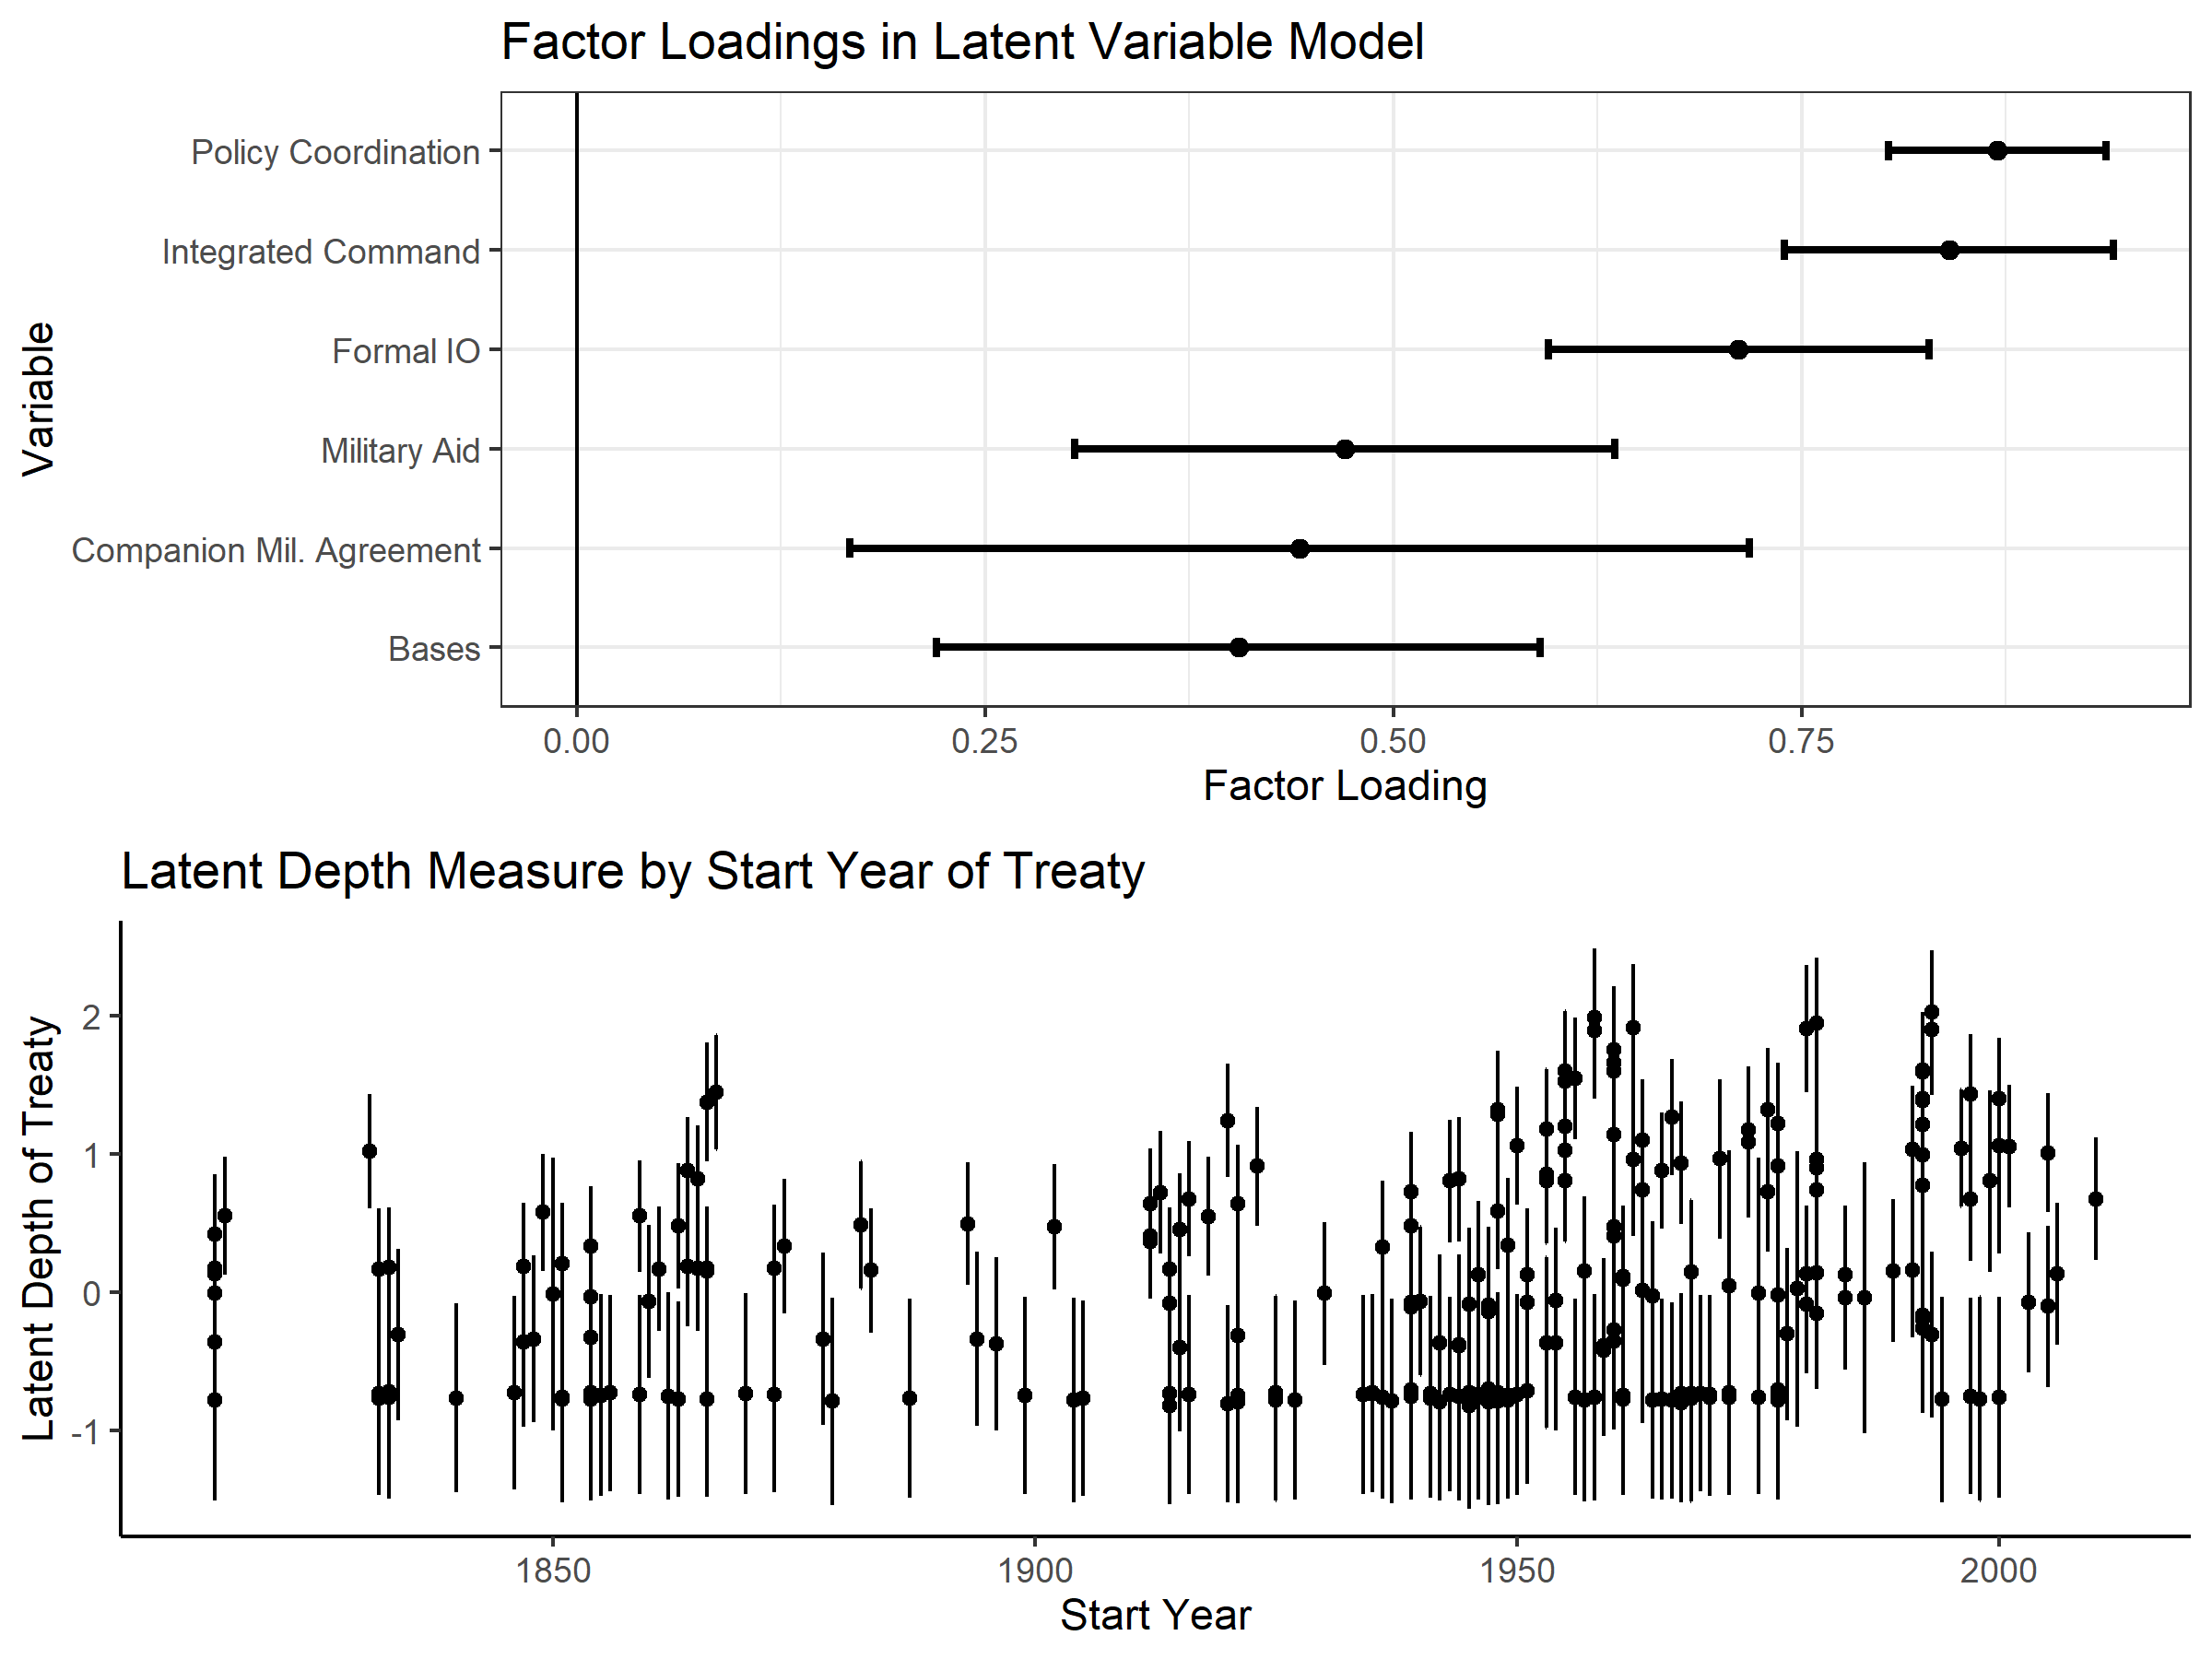
\includegraphics[width=0.95\textwidth]{../figures/loadings-measure.png}
\caption{Factor loadings and posterior distributions of the latent alliance treaty depth measure. Estimates from a semiparametic mixed factor analysis of offensive and defensive ATOP alliances from 1816 to 2007.}
\label{fig:loadings-measure}
\end{figure}


% discuss/justify the loadings
These factor loadings are sensible. 
Defense policy coordination, peacetime integrated command structures and formal organizations all draw alliance members into closer peacetime defense cooperation. 
The other variables do not require as much direct cooperation, with the potential exception of bases.
Although bases are costly, they also serve multiple functions and may not require as much direct cooperation. 
In addition to deterrence and increasing alliance credibility, states often use basing obligations to project power, so bases are used for other purposes besides promoting cooperation between allies, while the other factors provide for more direct cooperation.  


The measurement model predicts the treaty depth of each alliance using the factor loadings. 
The bottom panel of \autoref{fig:loadings-measure} summarizes the posterior distributions of the latent treaty depth measure for every alliance in the data. 
There is substantial variation in alliance treaty depth. 
Around half of all alliance treaties have some depth, and depth varies widely across alliances.
In the analysis, I measure treaty depth using the mean of the latent depth posterior for each alliance. 
The posterior mean captures the central tendency of latent treaty depth, and I show in the appendix that results are robust to accounting for uncertainty in the latent measure. 


The key independent variable is an ordinal indicator of electoral democracy in the most capable alliance member during the year of alliance formation. 
I use the the Lexical Index of Electoral Democracy (LIED) \citep{Skaaningetal2015} to measure electoral competition.
This ordinal measure assesses the extent of electoral democracy in a country based on six components and ranges from zero to six.  
States with no elections of any kind have an index score of zero, while single-party elections receive score a one. 
Multiparty elections for legislature or executive roles that fall short of a minimum competition threshold score a two or three. 
States with minimally competitive multiparty elections for executive and legislative roles have an index score of four, and scores of five and six come from expanding the franchise.

I retain the full range of the electoral index of democracy for two reasons.\footnote{In the appendix, I report findings with a dummy indicator of full electoral democracy, which produces similar inferences.}
First, unlike some measures of democracy, the LIED scale isolates the key concept of my argument.
Furthermore, the order of the scale places competitive elections before full suffrage, in contrast to other measures of electoral democracy, which give participation and electoral institutions equal weight. 
Widespread participation is only meaningful if leaders face some risk of removal through elections.


After measuring the lexical index for each country in an alliance, I identify the alliance leader.   
I code the alliance leader as the state with the largest composite index of national capabilities (CINC) score \citep{SingerCINC1988}, and measure their LIED score in the year the alliance formed.
The LIED of the most capable state therefore emphasizes the influence of the most capable alliance member and the prevalence of electoral democracy in that state.


I also measure executive constraints to examine whether it reduces treaty depth. 
Constraints are also positively associated with electoral democracy.
I set an executive constraints dummy equal to one if the executive constraints concept in the Polity data codes a state as having executive parity or subordination to other branches of government.
85 of the 289 alliances have such executive constraints on the leader of the most capable state.



\subsection{Estimation Strategy}



I use several statistical models to examine how democratic political institutions affect treaty depth.
I employ include a variety of regression approaches including a two-stage sample selection model. 

Modeling depth is complicated because the latent measure is skewed.
To facilitate model fitting, I rescaled latent depth to range between zero and one and modeled it with a beta distribution.\footnote{I also considered log-logistic, Dagum and inverse Gaussian distributions for the outcome, but AIC and residuals showed that the beta distribution gave the best model fit.}
The flexibility of the beta distribution helps predict mean latent depth.\footnote{Using a beta distribution for the depth outcome also facilitates fitting models that account for uncertainty in the latent measure, which I include in the appendix.} 
I also fit OLS, skew-t and skew-cauchy models of treaty depth without any rescaling.
The alliance leader democracy measures are the key independent variables in all these model specifications. 


In the regression models, I control for several correlates of treaty design and democratic institutions of the alliance leader. 
Key controls include dummy indicators of asymmetric alliances between non-major and major powers and symmetric alliances between major powers \citep{Mattes2012}\footnote{This leaves symmetric alliances between major powers as the base category for these two binary variables.} as well as the average threat among alliance members at the time of treaty formation \citep{LeedsSavun2007}. 
I also control for foreign policy similarity using the minimum value of Cohen's $\kappa$ in the alliance \citep{Hage2011}.
I draw on the ATOP data \citep{Leedsetal2002}, to adjust for for asymmetric treaty obligations, the number of alliance members and whether any alliance members were at war. 
To capture the role of issue linkages in facilitating alliance agreements and credible commitment \citep{Poast2012, Poast2013}, I include a dummy indicator of whether the alliance made any economic commitments. 
I also include an indicator of unconditional military support, which is correlated with democracy \citep{Chibaetal2015} and perhaps treaty depth. 
I adjust for a count of foreign policy concessions in the treaty, because concessions facilitate agreement in alliance negotiations \citep{Johnson2015}. 
Last, the model accounts for the role of time and the international context by using a non-linear smoothed term for the start year of the alliances to captures shift in the prevalence of deep or unconditional alliances over time.\footnote{I also check whether findings about democracy are driven the United States. See the appendix for results with an additional control for U.S. membership, which are similar to the inferences below.}



\section{Results}


I find that electoral democracy in the most capable alliance member leads to deep alliance treaties, starting with descriptive statistics. 
First, alliances where the leading alliance member had full electoral democracy were deeper on average, as the top panel of \autoref{fig:raw-data} shows. 
Many alliances with a democratic leader and treaty depth formed after 1945, but there are alliances before World War II that also fit this pattern. 

\begin{figure}[hbtp]
\centering
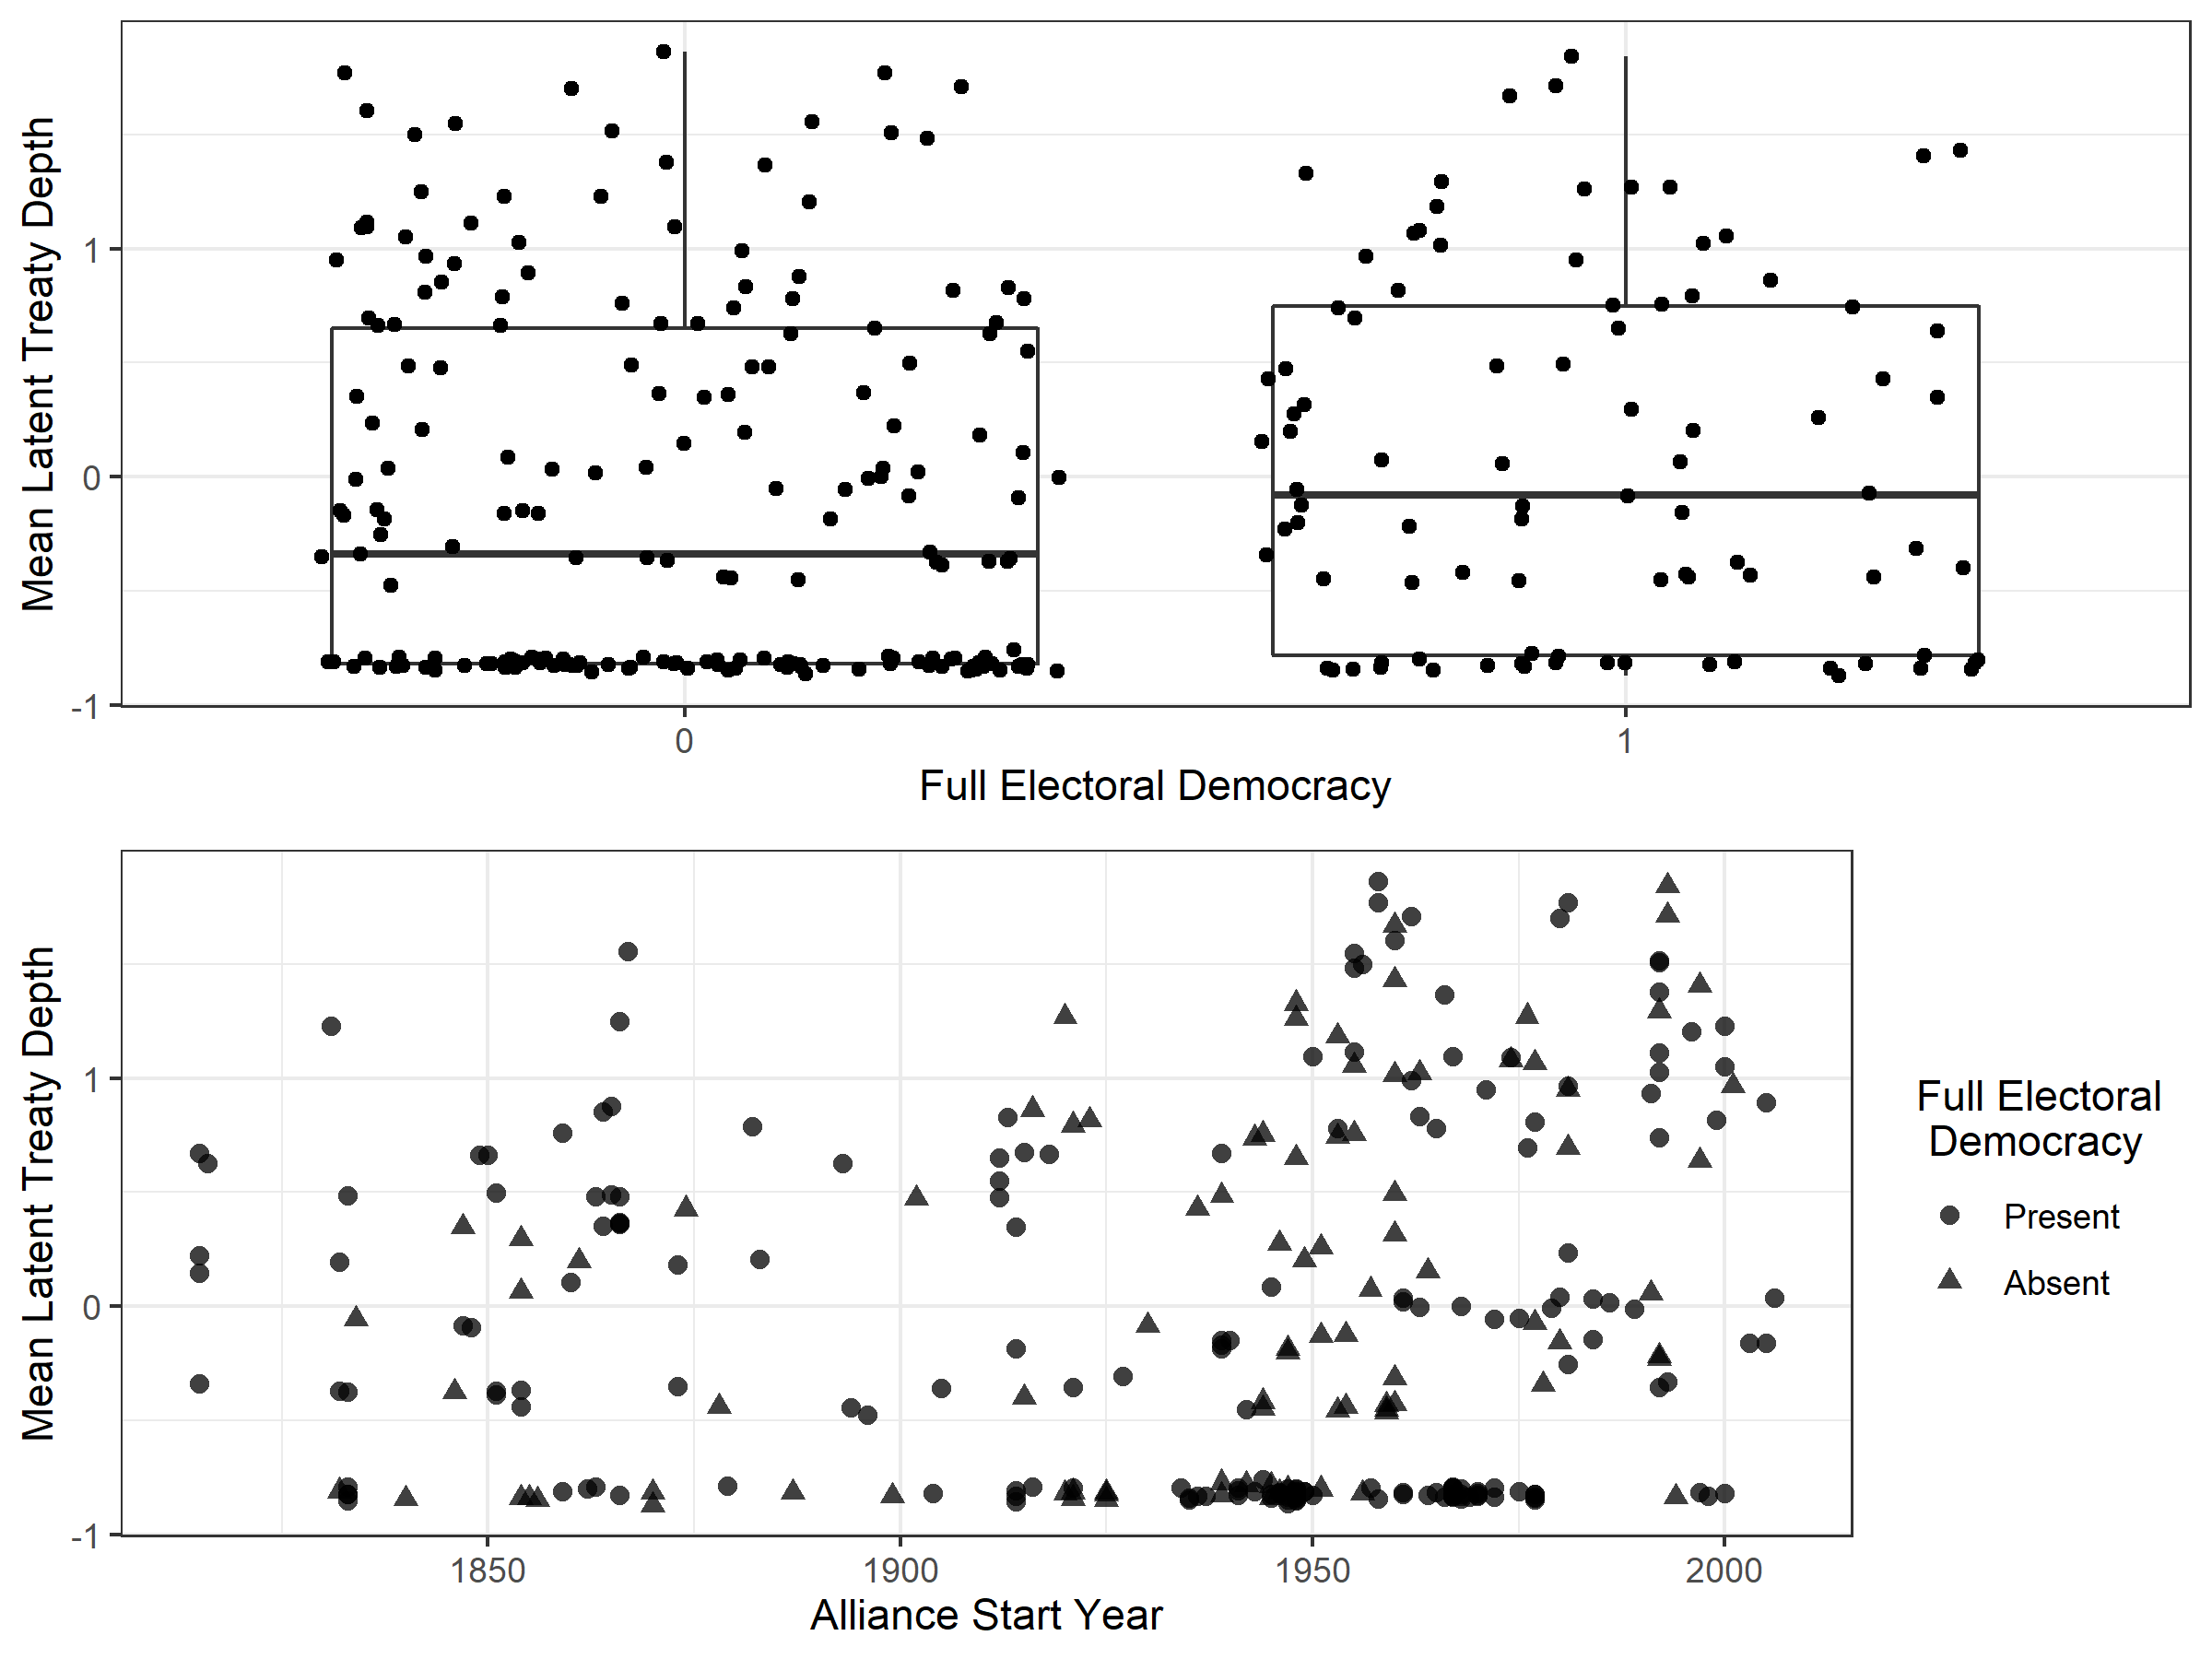
\includegraphics[width=0.95\textwidth]{../figures/raw-data.png}
\caption{Summary of raw data for alliance treaty depth and competitive elections. The top panel shows a boxplot with the distribution of mean latent treaty depth under alliances where the most capable member high electoral democracy, and alliances where the leader does not have electoral competition. The bottom panel plots mean latent treaty depth over time, and marks alliances with competitive elections in the most capable state with triangular points. }
\label{fig:raw-data}
\end{figure}


The raw data in \autoref{fig:raw-data} does not adjust for potential confounding factors, however. 
\autoref{tab:reg-est} presents coefficient estimates from a series of beta regression models. 
In the first model, the most capable alliance member's polity score is the key independent variable. 
The second model uses the lexical index of electoral democracy and executive constraints dummy as the key independent variables.  
The third model estimates the same model on alliances before 1945. 
The final model estimates the association between electoral democracy, executive constraints, and treaty depth among alliances after 1945. 


These estimates are broadly consistent with the argument. 
The net effect of more democratic institutions is to increase treaty depth, as the alliance leader polity estimate shows. 
Model 2 then shows that this is the result of electoral democracy, as increasing electoral democracy encourages alliance leaders to form deep alliances. 
Executive constraints has the opposite effect on alliance treaty design and reduces treaty depth. 
Although the effects are in the expected direction among alliances before 1945, the estimates are weaker and more uncertain. 
Model 4 shows that the pattern of electoral democracy, executive constraints and treaty depth is more pronounced after 1945. 


\begin{table}[!htbp] \centering 
 \resizebox{.95\textwidth}{!}{
\begin{tabular}{@{\extracolsep{5pt}}lcccc} 
\\[-1.8ex]\hline 
\hline \\[-1.8ex] 
 & \multicolumn{4}{c}{\textit{Dependent variable:}} \\ 
\cline{2-5} 
\\[-1.8ex] & \multicolumn{4}{c}{Latent Depth (rescaled)} \\ 
\\[-1.8ex] & (1) & (2) & (3) & (4)\\ 
\hline \\[-1.8ex] 
 Alliance Leader Polity & 0.025$^{}$ &  &  &  \\ 
  & (0.004, 0.046) &  &  &  \\ 
  Lexical Index of Democracy &  & 0.209$^{}$ & 0.113 & 0.229$^{}$ \\ 
  &  & (0.115, 0.303) & ($-$0.065, 0.291) & (0.110, 0.348) \\ 
  Executive Constraints &  & $-$0.797$^{}$ & $-$0.416 & $-$0.987$^{}$ \\ 
  &  & ($-$1.241, $-$0.353) & ($-$1.137, 0.306) & ($-$1.635, $-$0.339) \\ 
  Economic Issue Linkage & $-$0.187 & $-$0.214 & 0.286 & $-$0.344 \\ 
  & ($-$0.510, 0.137) & ($-$0.533, 0.104) & ($-$0.175, 0.747) & ($-$0.781, 0.093) \\ 
  Unconditional Support & 0.439$^{}$ & 0.424$^{}$ & 0.064 & 0.516$^{}$ \\ 
  & (0.133, 0.746) & (0.120, 0.729) & ($-$0.450, 0.578) & (0.139, 0.893) \\ 
  Foreign Policy Concessions & $-$0.012 & $-$0.069 & 0.109 & $-$0.200$^{}$ \\ 
  & ($-$0.176, 0.153) & ($-$0.233, 0.094) & ($-$0.118, 0.336) & ($-$0.439, 0.038) \\ 
  Number of Members & 0.017 & 0.034$^{}$ & $-$0.012 & 0.068$^{}$ \\ 
  & ($-$0.010, 0.044) & (0.007, 0.061) & ($-$0.056, 0.031) & (0.030, 0.106) \\ 
  Wartime Alliance & $-$0.187 & $-$0.017 & $-$0.069 & $-$0.134 \\ 
  & ($-$0.566, 0.192) & ($-$0.394, 0.360) & ($-$0.468, 0.331) & ($-$1.117, 0.850) \\ 
  Asymmetric Obligations & 0.153 & 0.241 & 0.066 & 0.345 \\ 
  & ($-$0.194, 0.500) & ($-$0.104, 0.586) & ($-$0.335, 0.468) & ($-$0.252, 0.941) \\ 
  Asymmetric Capability & 0.393 & 0.333 & 0.558$^{}$ & 0.121 \\ 
  & ($-$0.077, 0.863) & ($-$0.134, 0.800) & (0.092, 1.024) & ($-$0.343, 0.586) \\ 
  Non-Major Only & 0.160 & 0.138 & 0.252 &  \\ 
  & ($-$0.358, 0.677) & ($-$0.376, 0.651) & ($-$0.330, 0.834) &  \\ 
  Average Threat & 0.874$^{}$ & 0.965$^{}$ & 1.643$^{}$ & 0.653 \\ 
  & (0.038, 1.710) & (0.132, 1.798) & (0.419, 2.867) & ($-$0.487, 1.793) \\ 
  Foreign Policy Disagreement & 0.295 & 0.215 & 0.440 & 0.043 \\ 
  & ($-$0.186, 0.775) & ($-$0.256, 0.686) & ($-$0.163, 1.044) & ($-$0.712, 0.798) \\ 
  Post 1945 & 0.208 & 0.196 &  &  \\ 
  & ($-$0.169, 0.584) & ($-$0.175, 0.566) &  &  \\ 
  Constant & $-$1.658$^{}$ & $-$1.956$^{}$ & $-$2.536$^{}$ & $-$1.347$^{}$ \\ 
  & ($-$2.399, $-$0.916) & ($-$2.741, $-$1.170) & ($-$3.511, $-$1.562) & ($-$2.374, $-$0.320) \\ 
 \hline \\[-1.8ex] 
Observations & 276 & 276 & 118 & 158 \\ 
Log Likelihood & 56.692 & 63.188 & 44.319 & 35.603 \\ 
\hline 
\hline \\[-1.8ex] 
\textit{Note:}  & \multicolumn{4}{r}{95\% Confidence Intervals in Parentheses.} \\ 
\end{tabular} 
}
  \caption{Beta regression estimates of the association between alliance leader democracy and treaty depth from 1816 to 2007.} 
  \label{tab:reg-est} 
\end{table} 

Inferences about the control variables are also interesting.
More alliance members and asymmetric capability both increase depth, as does external threat.
The association between threat and depth is stronger before World War II, while multilateral alliances after 1945 tend to be deeper. 
Unconditional military support and treaty depth are positively correlated, especially after 1945. 


To assess the substantive impact of elections, I estimated the difference between different levels of electoral democracy and no electoral democracy using simulated coefficient vectors from the model. 
In the scenarios, I held all other variables at their mode or median and varied the values of electoral competition and treaty depth. 
I then varied the lexical index of electoral democracy across its full range and predicted treaty depth in seven hypothetical alliances. 
I also varied the presence or absence of electoral constraints. 
\autoref{fig:results-diff} plots the difference in predicted treaty depth or the probability of unconditional military support between fourteen hypothetical alliances with different combinations of executive constraints and electoral democracy and a baseline scenario without either democratic institution. 


\begin{figure}[hbtp]
\centering
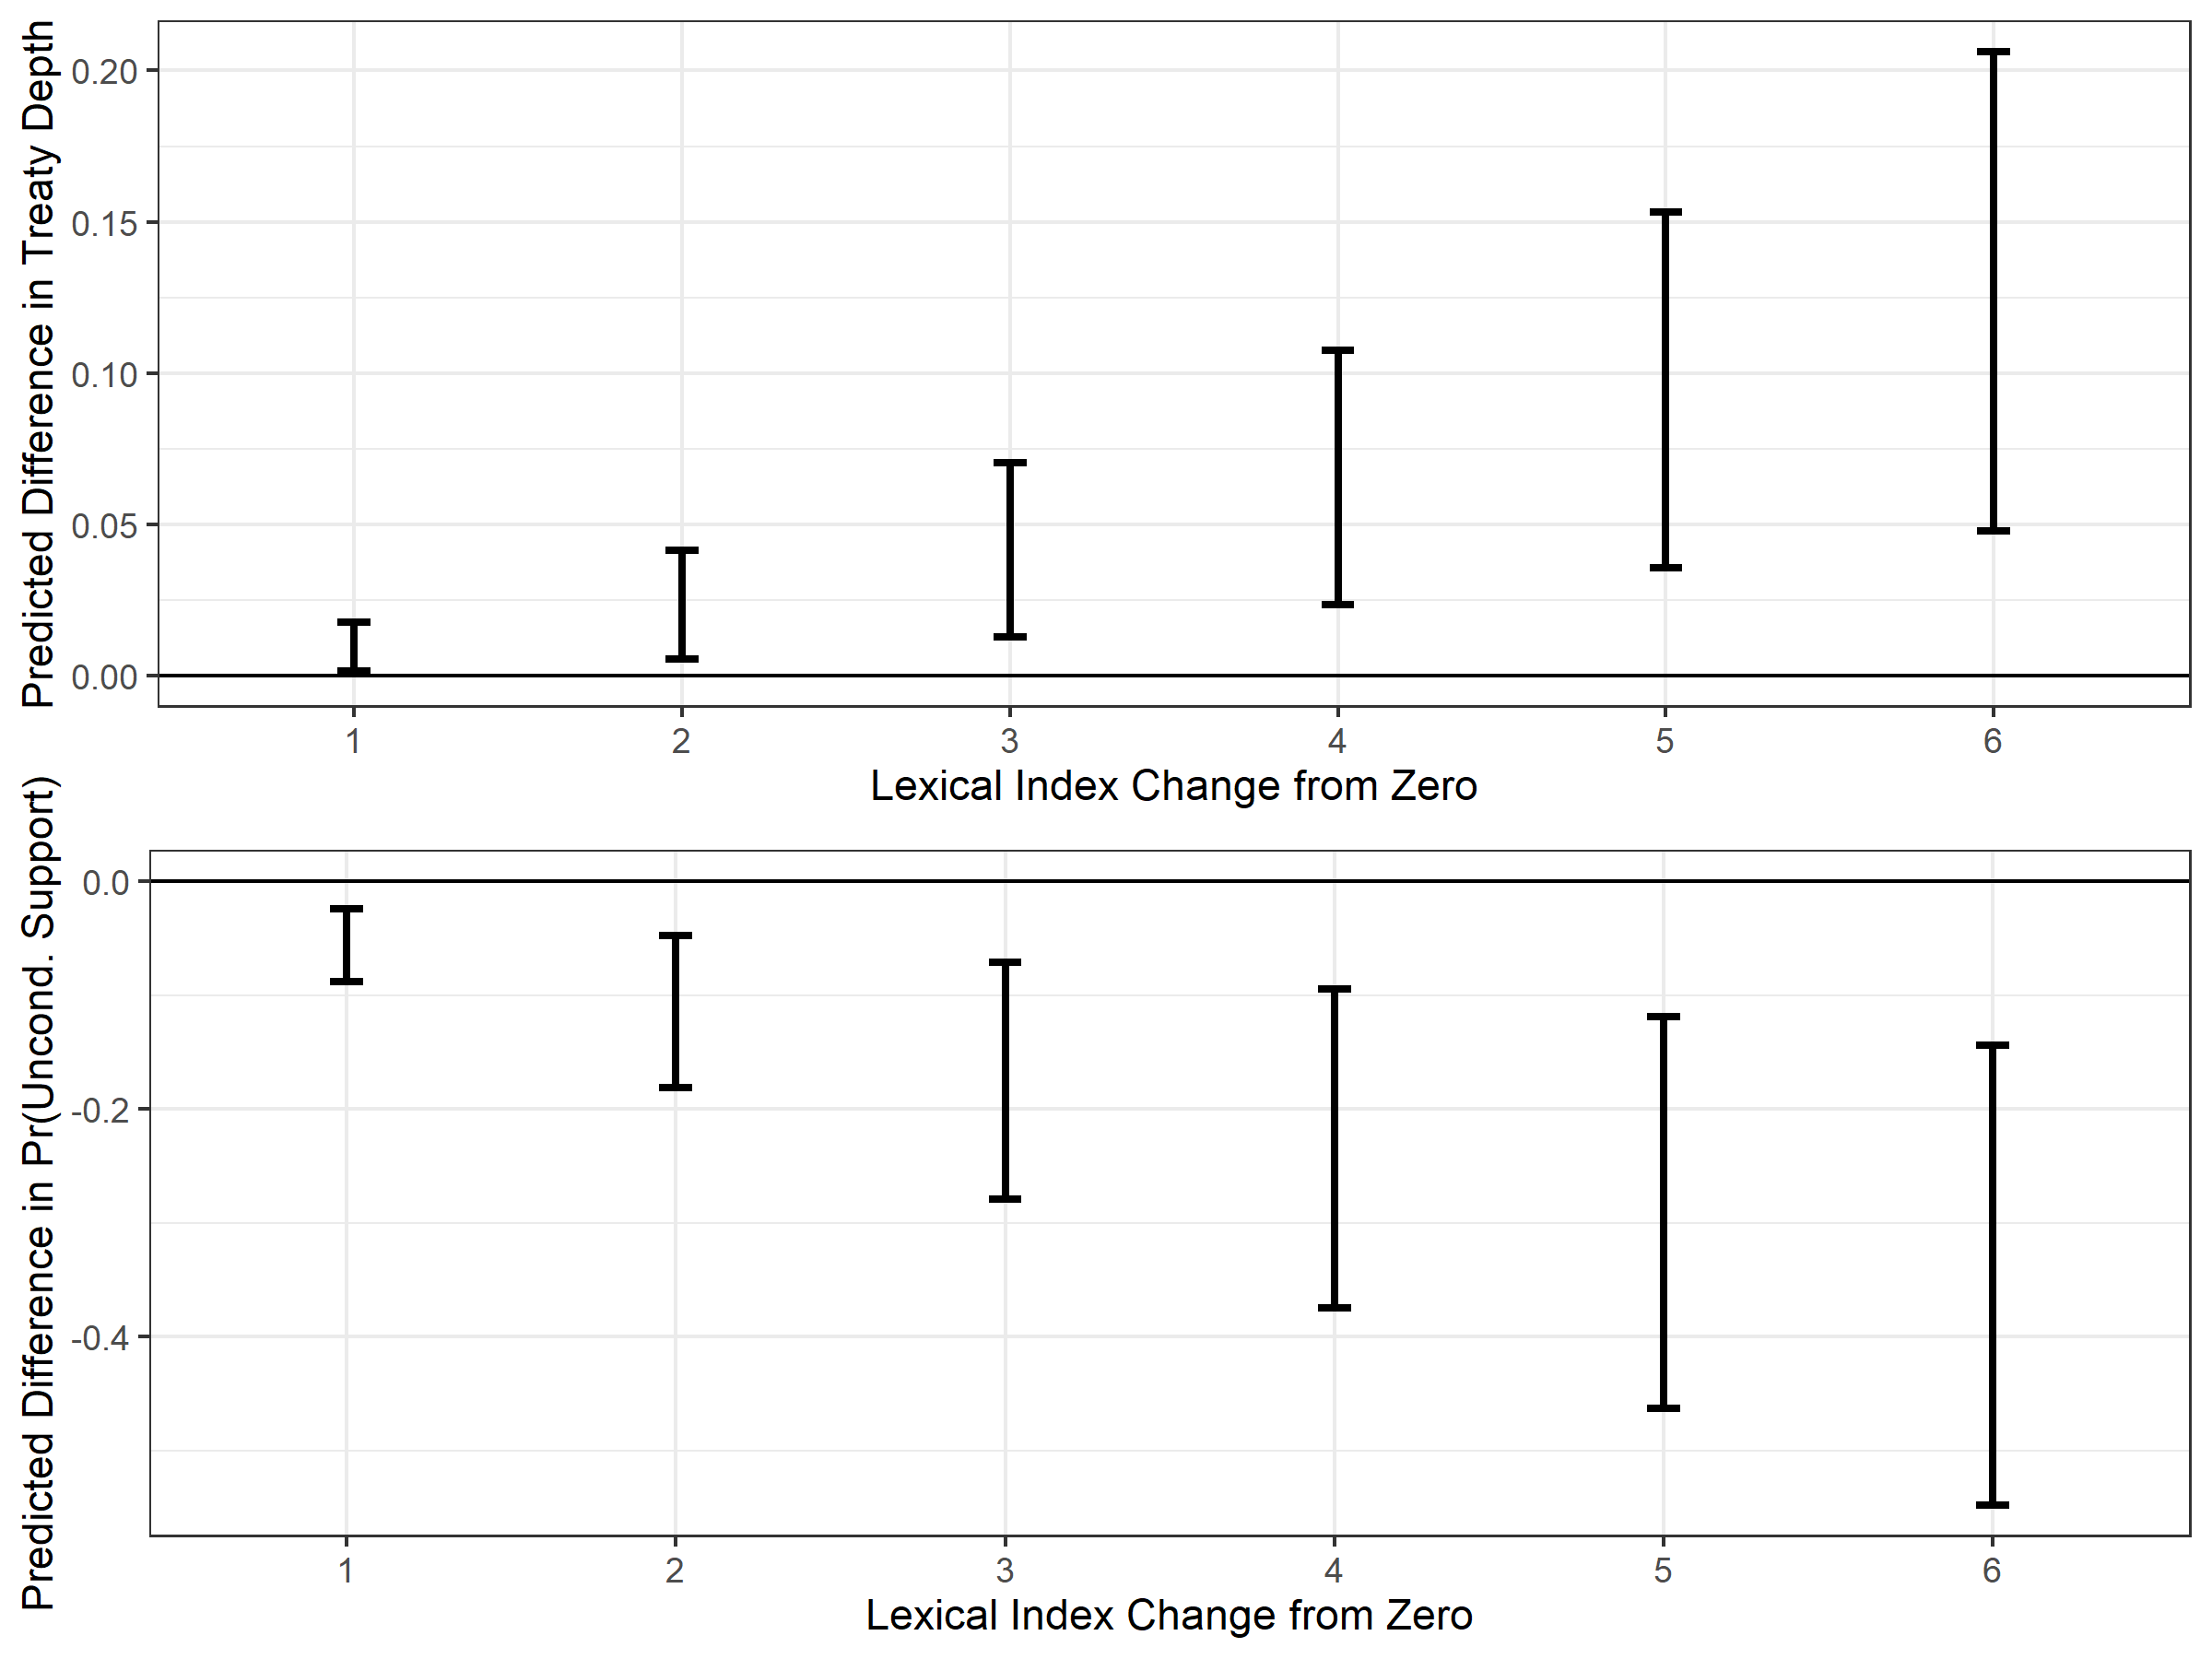
\includegraphics[width=0.95\textwidth]{../figures/results-diff.png}
\caption{Predicted difference in treaty depth and the probability of unconditional military support relative to a hypothetical alliance where the most capable state has no electoral democracy. Each scenario plots the estimated difference in treaty depth. All other variables held at their mean or median, expect for executive constraints, which varies between zero and one.}
\label{fig:results-diff}
\end{figure}


Greater electoral democracy has a clear substantive impact on alliance treaty depth, but when executive constraints are present, only full electoral democracy clearly increases treaty depth. 
Alliances where the most capable state has full electoral democracy have between .01 and .27 more latent depth relative to a hypothetical alliance with no democratic institutions when executive constraints are also present all else equal.
As rescaled depth ranges between zero and one, these are meaningful substantive effects, though the magnitude of the electoral democracy effect includes relatively small and large and effects. 


\autoref{fig:results-diff} shows that the extent of electoral democracy affects alliance treaty design.
When alliance leaders face electoral scrutiny, they are more inclined to form deep alliances. 
Executive constraints may somwhat restrict depth, however.
Thus, it takes full electoral democracy to produce the net positive association between democracy and alliance treaty depth. 


My argument implies that a selection process is present, however. 
Observed treaty depth reflects situations where leaders have voter approval to form an alliance.
But observed alliances are not a random sample--- they are the result of successful negotiations \citep{Poast2019a}. 
In the next section, I check the robustness of these results to accounting for non-random selection into alliances. 


\subsection{Selection Model of Treaty Depth} 


Observed alliances are the result of negotiations between potential members, so the set of observed alliances is not a random sample.
Rather, alliance members overcame the many obstacles to alliance formation \citep{Poast2019a}.  
In this section, I account for non-random alliance formation using a hurdle model of observed alliances after combining a stratified random sample of non-allied groups of states with observed alliances. 
This research design produces similar inferences: electoral democracy in the most capable alliance member increases treaty depth. 


My research design for this robustness check follows established procedures for dealing with selection into alliances and treaty design. 
I followed the suggestions of \citet{Poast2010} for using k-adic data, because some alliances have more than two members. 
First I constructed a random sample of groups of states that could have formed an alliance in each year, but did not \citep{FordhamPoast2014}.
Then I took a stratified sample of the non-allied k-ads to include five times as many non-allied observations as alliance observations for each observed value of alliance size. 
For example, there are 215 bilateral alliances, so I sampled 1075 non-allied bilateral groups. 
There is only one alliance with 34 members, so I added five non-alled k-ads with 34 members. 
Finally, I summarized key characteristics of these non-allied k-ads, including average Polity score, the electoral democracy of the most capable member, the number of members, mean threat, asymmetric capability, and wartime, and merged the non-allied data with the observed alliance data. 


To model alliance treaty alliance design, I emulated the research design of \citet{Chibaetal2015}, who estimated a hurdle model to assess whether democracies were more likely to offer conditional obligations.
Hurdle models have two stages or parts which account for non-random selection into alliances.
A first stage model predicts which observations clear the hurdle to a second stage with non-zero outcome values. 
Observed alliances are the set of observations that cleared the hurdle and have an alliance treaty. 
Unlike a sample selection model, the second stage in a hurdle model is logically undefined, which is how alliance treaty design works.\footnote{Hurdle models also do not require an exclusion restriction for identification.} 
Unless states overcome the barriers to alliance formation, no agreed treaty content exists. 


Unlike \citet{Chibaetal2015}, however, I examine a continuous measure of alliance treaty design with latent depth. 
Therefore, I estimate a Bayesian gamma hurdle model using the BRMS package for \textsf{R}, which employs STAN for fully Bayesian inference \citep{Buerkner2017}.
To have zero values for the outcome at the hurdle stage and positive values for the gamma-distributed outcome, I adjusted the latent depth measure by adding one, which shifted the distribution onto uniformly positive values. 


In both models, I use average democracy, alliance leader constraints and democracy, mean threat, asymmetric capability, wartime, and year varying intercepts to predict whether the group of states clears the alliance formation hurdle.
In the second stage, I use electoral competition and executive constraints in the most capable alliance member, the number of members, mean threat, dummy indicators of asymmetric capability or non-major power only membership, wartime and year varying intercepts to model treaty depth and alliance formation. 


After accounting for non-random alliance formation with the hurdle model, I find partially similar results. 
\autoref{fig:results-hurdle} plots the marginal effect of the two democratic institution measures based on the hurdle model estimates. 
This figure shows the predicted marginal effect of electoral democracy and executive constraints in the alliance leader on shifted treaty depth, along with 95\% credible intervals.
Electoral democracy in the most capable alliance member increases treaty depth, but the effect of executive constraints is weaker than the single-equation results.  


\begin{figure}
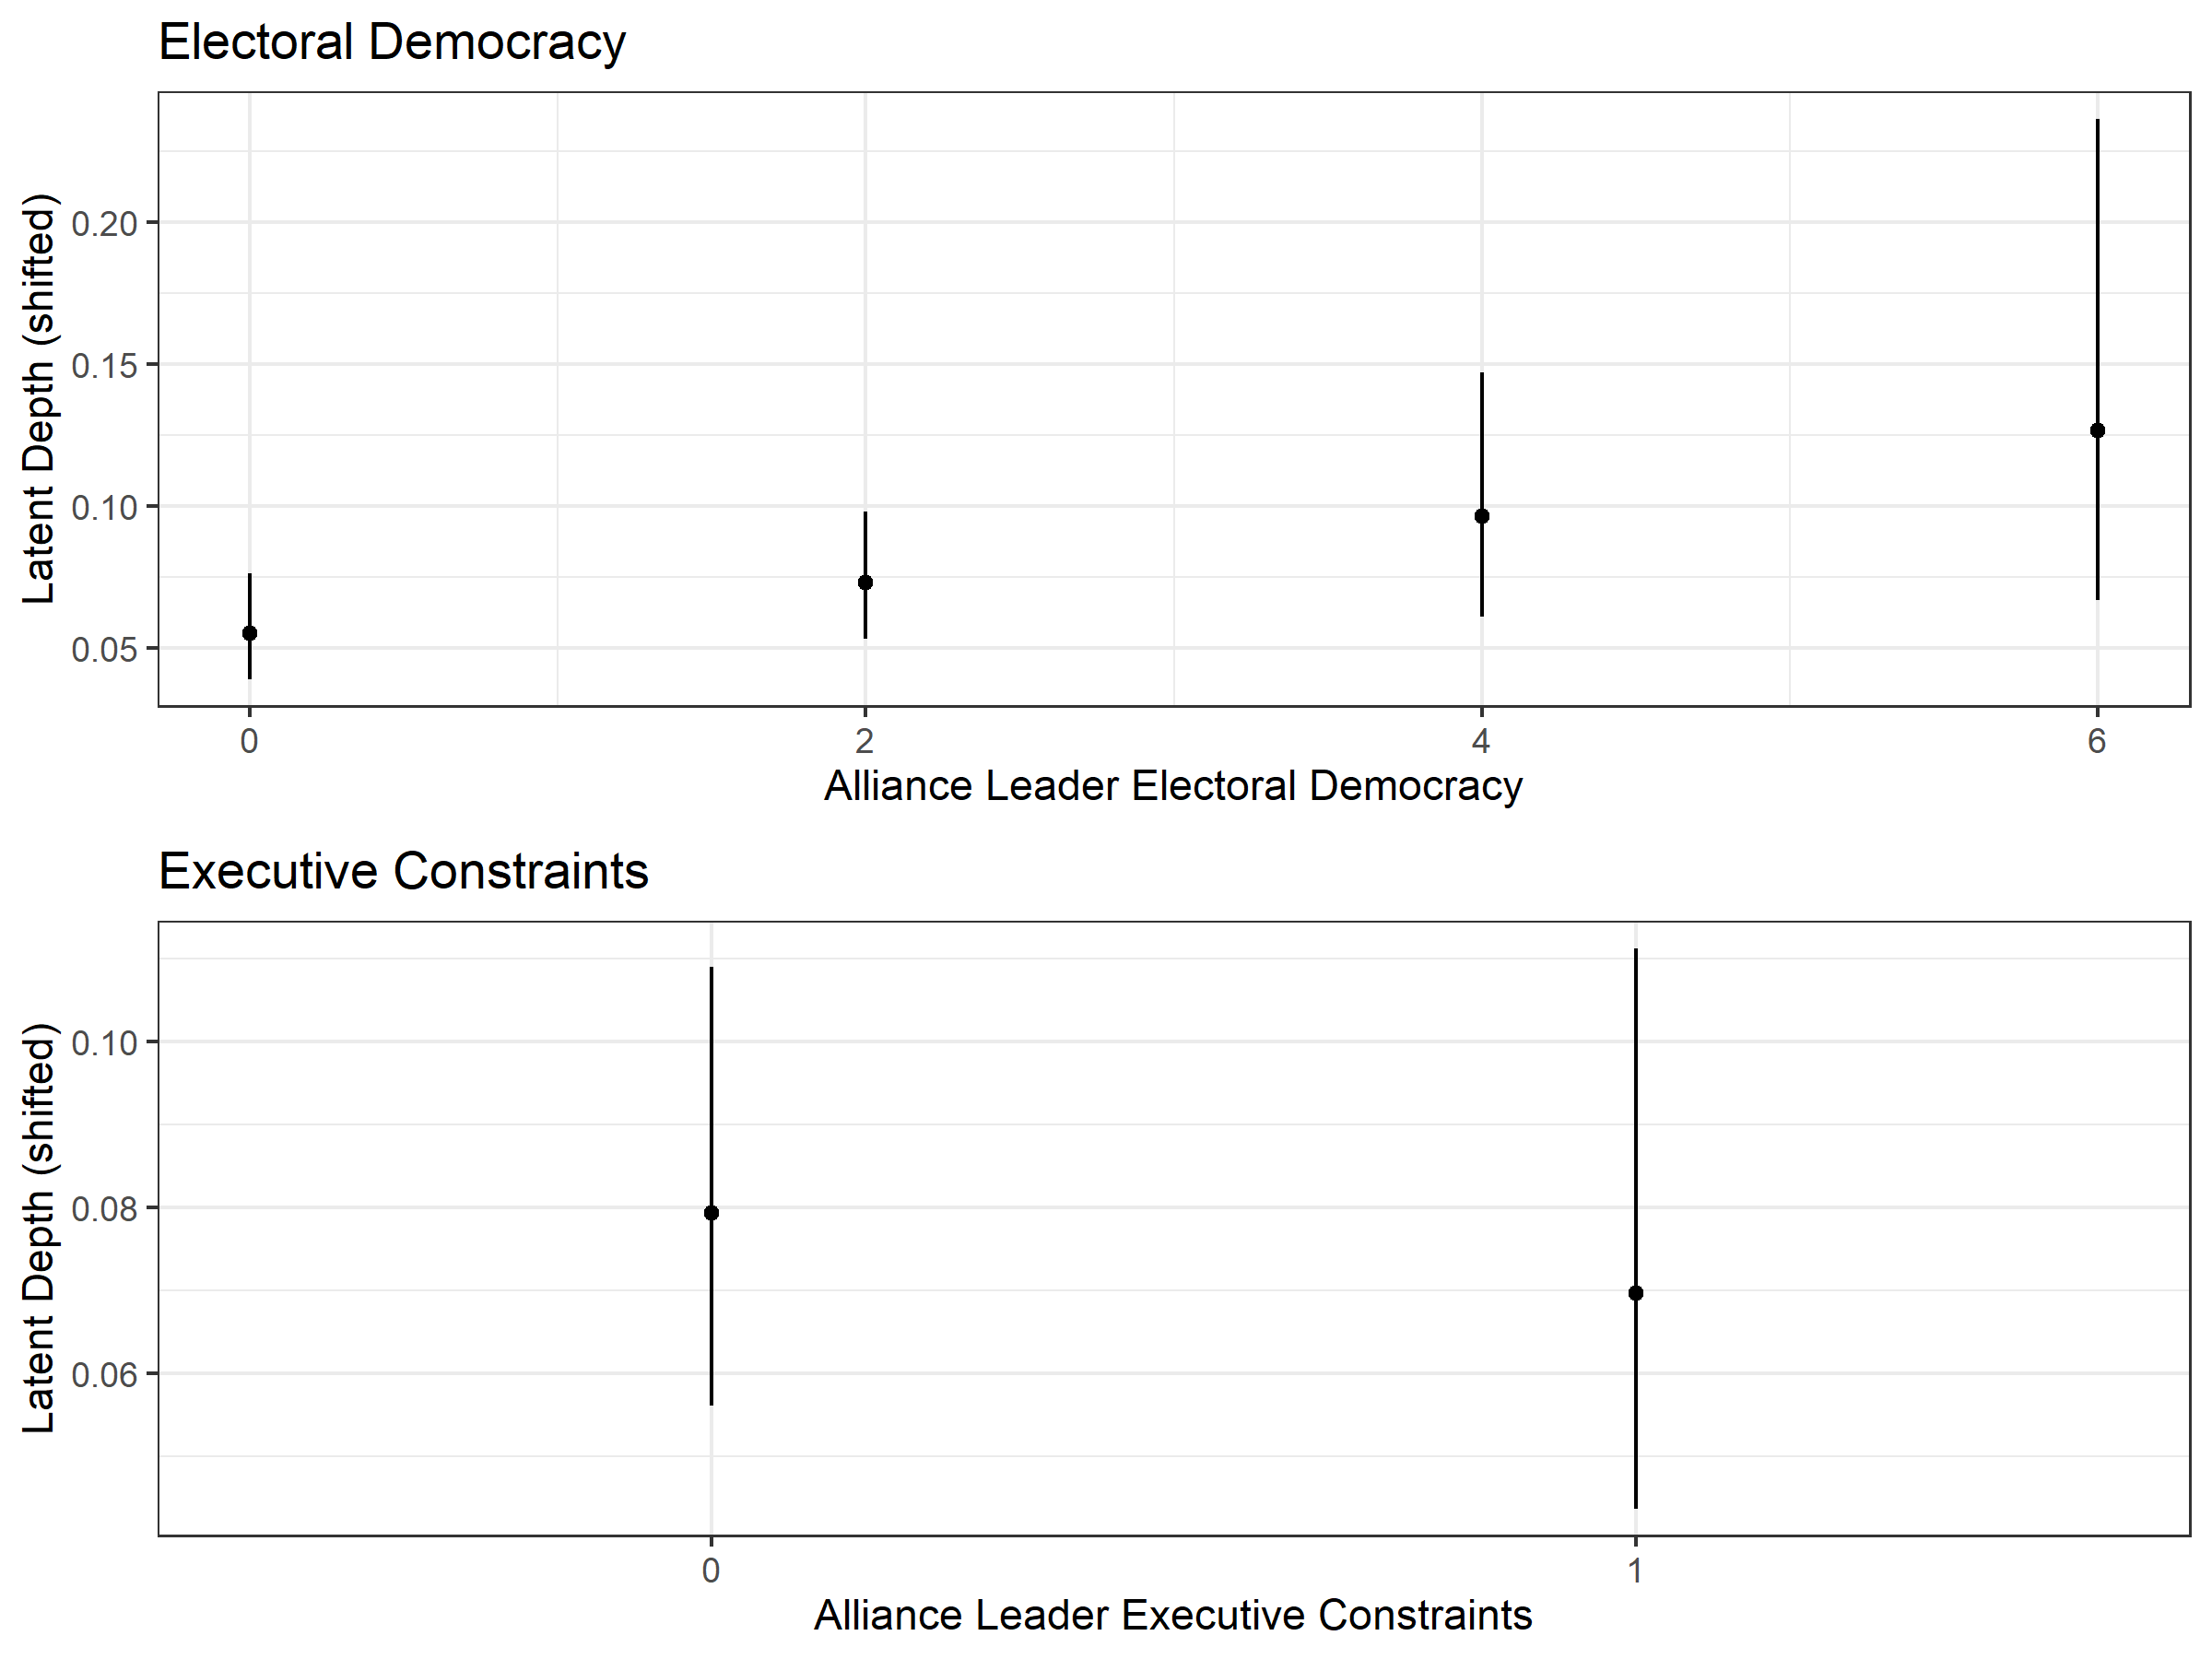
\includegraphics[width=.95\textwidth]{../figures/results-hurdle.png}  
\caption{Predicted changes in treaty depth by electoral democracy and executive constraints in the most capable alliance member when the treaty formed. Estimates are based on a hurdle model of alliance treaty depth. The line marks predicted values, and the shaded areas encapsulate the 95\% credible interval. Predictions hold all other variables constant.}
\label{fig:results-hurdle}
\end{figure}


Even after considering non-random alliance formation, electoral democracy encourages deep alliances. 
When democratic leaders successfully pursue an alliance agreement, they then try to buttress the alliance against leadership turnover through depth. 
After accounting for non-random selection into alliances, executive constraints are not associated with shallower alliances.
Whether the opposition cannot or does not check alliance formation, they have limited influence over treaty depth. 


The results of these statistical models imply that democratic institutions impact alliance treaty design. 
Electoral democracy pushes alliance leaders to form deep alliances. 
After accounting for non-random selection into observed alliances, executive constraints do not check treaty depth. 
To illustrate the theoretical process more directly, I now examine the North Atlantic Treaty Organization (NATO).



\subsection{NATO Treaty Design}


I use NATO to show the theoretical mechanisms for two reasons. 
First, the process behind NATO applies to multiple alliances, as other US alliance treaties have similar designs. 
Second, NATO is the most important alliance in international politics, as it has a crucial role in the structure of international relations by tying the United States to Europe. 
Because NATO is an exceptionally durable and consequential alliance, understanding how the treaty formed is worthwhile. 


After World War II, the United States sought a way to protect Europe from the USSR. 
Despite acute security concerns, criticism from opposition politicians led the United States to offer conditional military support. 
As \citet{Poast2019a} details, NATO members disagreed over how to define the North Atlantic area, especially with reference to France's Algerian colony and Italy, as the North Atlantic area was a key condition on military support. 
Furthermore, active military support from NATO members depends on domestic political processes.\footnote{\citet{Benson2012} calls this commitment a ``probablistic'' obligation.} 
Isolationists in the US Senate feared that an alliance would force automatic intervention, bypassing the power of Congress to declare war and engaging the US in unwanted conflicts \citep[pg. 280-1]{Acheson1969}.
Therefore, Article V of the NATO treaty states that if one member is attacked the others ``will assist the Party or Parties so attacked by taking forthwith, individually and in concert with the other Parties, \emph{such action as it deems necessary} (emphasis mine).'' 
Military support was and is not guaranteed by Article V, and US policymakers used this limited commitment to sell NATO to the public. 
In a March 1949 press release to the public, Secretary of State Dean Acheson said that Article V ``does not mean that the United States would automatically be at war if one of the nations covered by the Pact is subject to armed attack'' \citep{Acheson1949}.
This claim and the emphases of the press release show that promises of military support were salient to the US public, which was a key rationale for limited promises of military support. 


Military support from Article V did not assuage European fears that if the Soviets invaded, the United States would abandon them.
To increase the credibility of NATO, the United States took other measures.  
A 1951 presentation by Dean Acheson to Dwight Eisenhower argued that European allies ``fear the inconstancy of United States purpose in Europe. ... These European fears and apprehensions can only be overcome if we move forward with determination and if we make the necessary full and active contribution in terms of both military forces and economic aid'' \citep[pg. 3]{Acheson1951}. 
To start, the US supported the Atlantic Council, an international organization and the main source of depth in the NATO treaty. 
The United States used the Atlantic Council to coordinate collective defense and increase the perceived reliability of the alliance. 
By investing in the Atlantic Council and related joint military planning, the United States addressed European fears of abandonment. 
For example, US officials thought that the British Foreign Minister viewed US provision of a supreme commander in Europe as ``a stimulus to European action'' in NATO \citep{Acheson1950}. 


Policymakers then used defense cooperation with allies to justify NATO participation by arguing that it would facilitate more efficient defense spending. 
In an interview with NBC on March 29, Ambassador at Large Philip Jessup argued that ``One defense program is cheaper and more effective than a dozen national programs. It entails the pooling of information, a joint defense strategy and a pooling of military resources for defense.''
This claim was meant to assuage concerns that NATO would reduce the US ``peace dividend'' after World War II. 


NATO also illustrates that executive constraints might limit treaty depth. 
Many Senators also opposed military aid to Europe \citep[pg 285]{Acheson1969}. 
Thus, legislative constraints on the executive branch reduced the formal depth of NATO relative to what many ambassadors preferred \citep[pg 277]{Acheson1969}, which matches the statistical inference about executive constraints and treaty depth.  
Bilateral agreements on troop deployments thus became another instrument of reassurance. 
In 1950 the Germans formally requested clarification on whether an attack on US forces in Germany would be treated as an armed attack on the United States- and US policymakers said that it would \citep[pg. 395]{Acheson1969}.  
These bilateral arrangements and basing rights are not covered in the NATO treaty, but they added substantial depth.\footnote{This reveals a potential limitation of the statistical models.}  


% Sum up 
In NATO, electoral concerns and anticipation of opposition criticism led the United States to offer conditional military support, but did not inhibit deep military cooperation, which helped reassure European allies. 
Limits on the promises of military support were a salient part of public discussions in the NATO treaty, while the Atlantic Council had a smaller role in public discourse, and policymakers attempted to sell such cooperation as source of efficient defense spending. 
The Atlantic Council and associated bureaucracy are the formal core of substantial defense cooperation. 
NATO negotiations show how a democratic alliance leader used treaty depth to reassure their allies, rather than unconditional military support. 
In the next section, I summarize some implications of the results and offer concluding thoughts. 



\section{Discussion and Conclusion} 


% main evidence summary
In summary, the findings from the statistical models generate fairly consistent evidence for the hypotheses, and the NATO illustration suggests that the theoretical mechanisms are plausible. 
Across multiple models and measures, electoral democracy is positively correlated with treaty depth.  
Because depth is a less transparent source of alliance credibility, democratic leaders use depth to increase the credibility of alliance commitments, while avoiding more transparent credibility sources like unconditional military support.


% limitations
My argument and evidence have two limitations.
First, I only examine variation in formal treaty design. 
This omits treaty implementation, which can diverge from the formal commitment.   
Formal treaty depth often reflects practical depth, but it may understate some differences between alliances. 
Changes in realized alliance depth are a useful subject for future inquiry, but will require extensive data collection.
Second, I examine 280 alliances, so the sample size is limited. 
Inferences from small samples can be more sensitive to model and data changes. 


Shortcomings aside, this paper has four implications for scholarship. 
First, alliance treaty design is often driven by domestic political considerations. 
Attempts to remain in office and avoid opposition criticism in electoral politics encourage democratic leaders to design deep alliance treaties with conditional promises on military support. 


Second, different aspects of alliance treaty design are related \citep{FjelstulReiter2019}. 
As states attempt to make credible alliance commitments, they can employ a range of treaty obligations. 
Furthermore, the connection between depth and unconditional support varies with the international context. 
Thus, studying individual aspects of alliance treaty design in isolation leads to incomplete portrayals of the treaty design process. 


Third, democracies do not make fully limited alliance commitments with conditional obligations and no depth.
Even if democracies impose conditions on military support, treaty depth adds costly obligations.
As a result, democracies make robust alliance commitments in one way, and limited commitments in another. 


Last, some of the lessons from this work might apply to the design on international institutions in general \citep{DownesRocke1995, MartinSimmons1998, Koremenosetal2001, Thompson2010}.
In the same way that democracies use depth to support allies while managing electoral politics, democracies may undertake deep international commitments in ways that limit electoral scrutiny. 
The same mix of limited core obligations and deep cooperation may characterize other international institutions with democratic leadership. 


The findings raise at least two questions for future research.  
For one, they address debates about whether democracies make more credible commitments. 
Even if conditional military support reduces the credibility of democratic alliances, treaty depth has the opposite effect. 
The net effect of democracy on alliance credibility therefore includes conditions on military support, treaty depth, and the direct effect of democratic institutions and domestic politics. 
These three mechanisms may have competing or conditional effects, which could explain mixed findings about the credibility of democratic commitments \citep{Schultz1999, Leeds1999, Thyne2012, DownesSechser2012, PotterBaum2014}.
Future research should combine the components of democracy and democratic alliances to asses the net effect of democracy on credible commitment in international relations. 


Scholars should also consider how alliance treaty design varies across different types of autocracies. 
The extent and sources of political competition in autocracies varies widely. 
Differences in who selects leaders and what information those actors have about foreign policy \citep{Weeks2008} may help explain alliance treaty design.
For example, personalist leaders with few public or elite constraints on their foreign policy may design alliances with depth and unconditional military support. 
Single party states where leaders face an informed elite may prefer fully limited commitments with shallow and conditional obligations. 


In conclusion, electoral democracy encourages democracies to use treaty depth to increase the credibility of their alliances. 
Deep alliances reassure democracies' alliance partners while limiting electoral criticism of alliances. 
By shaping leaders' foreign policy audiences, domestic political institutions influence how states build credibility into alliance treaties.




 
\bibliography{../../../MasterBibliography} 





\end{document}
